% !TeX root = RJwrapper.tex
\title{Conversations in Time: Interactive Visualization to Explore Structured Temporal Data}
\author{by Earo Wang and Dianne Cook}

\maketitle

\abstract{%
Temporal data often has a hierarchical structure, defined by categorical variables describing different levels, such as political regions or sales products. The nesting of categorical variables produces a hierarchical structure. The \CRANpkg{tsibbletalk} package is developed to allow a user to interactively explore temporal data, relative to the nested or crossed structures. It can help to discover differences between category levels, and uncover interesting periodic or aperiodic slices. The package implements a shared \texttt{tsibble} object that allows for linked brushing between coordinated views, and a shiny module that aids in wrapping timelines for seasonal patterns. The tools are demonstrated using two data examples: domestic tourism in Australia and pedestrian traffic in Melbourne.
}

\hypertarget{introduction}{%
\section{Introduction}\label{introduction}}

Temporal data typically arrives as a set of many observational units measured over time. Some variables may be categorical, containing a hierarchy in the collection process, that may be measurements taken in different geographic regions, or types of products sold by one company. Exploring these multiple features can be daunting. Ensemble graphics (Unwin and Valero-Mora 2018) bundle multiple views of a data set together into one composite figure. These provide an effective approach for exploring and digesting many different aspects of temporal data. Adding interactivity to the ensemble can greatly enhance the exploration process.

This paper describes new software, the \CRANpkg{tsibbletalk} package, for exploring temporal data using linked views and time wrapping. We first provide some background to the approach based on setting up data structures and workflow, and give an overview of interactive systems in R. The section following introduces the \CRANpkg{tsibbletalk} package. We explain the mechanism for constructing interactivity, to link between multiple hierarchical data objects and hence plots, and describe the set up for interactively slicing and dicing time to wrap a series on itself to investigate periodicities.

\hypertarget{background-tidy-temporal-data-and-workflow}{%
\section{Background: tidy temporal data and workflow}\label{background-tidy-temporal-data-and-workflow}}

The \CRANpkg{tsibble} package (Wang, Cook, and Hyndman 2020) introduced a unified temporal data structure, referred to as a \texttt{tsibble}, to represent time series and longitudinal data in a tidy format (Wickham 2014). A \texttt{tsibble} extends the \texttt{data.frame} and \texttt{tibble} classes with the temporal contextual metadata: \texttt{index} and \texttt{key}. The \texttt{index} declares a data column that holds time-related indices. The \texttt{key} identifies a collection of related series or panels observed over the \texttt{index}-defined period, which can comprise multiple columns. An example of a \texttt{tsibble} can be found in the monthly Australian retail trade turnover data (\texttt{aus\_retail}), available in the \CRANpkg{tsibbledata} package (O'Hara-Wild, Hyndman, and Wang 2020c), shown below. The \texttt{Month} column holds year-months as the \texttt{index}. \texttt{State} and \texttt{Industry} are the identifiers for these 152 series, which form the \texttt{key}. Note that the column \texttt{Series\ ID} could be an alternative option for setting up the \texttt{key}, but \texttt{State} and \texttt{Industry} are more readable and informative. The \texttt{index} and \texttt{key} are ``sticky'' columns to a \texttt{tsibble}, forming critical pieces for fluent downstream temporal data analysis.

\begin{verbatim}
#> # A tsibble: 64,532 x 5 [1M]
#> # Key:       State, Industry [152]
#>   State                        Industry                 Serie~1    Month Turno~2
#>   <chr>                        <chr>                    <chr>      <mth>   <dbl>
#> 1 Australian Capital Territory Cafes, restaurants and ~ A33498~ 1982 Apr     4.4
#> 2 Australian Capital Territory Cafes, restaurants and ~ A33498~ 1982 May     3.4
#> 3 Australian Capital Territory Cafes, restaurants and ~ A33498~ 1982 Jun     3.6
#> 4 Australian Capital Territory Cafes, restaurants and ~ A33498~ 1982 Jul     4  
#> 5 Australian Capital Territory Cafes, restaurants and ~ A33498~ 1982 Aug     3.6
#> # ... with 64,527 more rows, and abbreviated variable names 1: `Series ID`,
#> #   2: Turnover
\end{verbatim}

In the spirit of tidy data from the \CRANpkg{tidyverse} (Wickham et al. 2019), the \textbf{tidyverts} suite features \texttt{tsibble} as the foundational data structure, and helps to build a fluid and fluent pipeline for time series analysis. Besides \CRANpkg{tsibble}, the \CRANpkg{feasts} (O'Hara-Wild, Hyndman, and Wang 2020b) and \CRANpkg{fable} (O'Hara-Wild, Hyndman, and Wang 2020a) packages fill the role of statistical analysis and forecasting in the \textbf{tidyverts} ecosystem. During all the steps of a time series analysis, the series of interest, denoted by the \texttt{key} variable, typically persist, through the trend modeling and also forecasting. We would typically want to examine the series across all of the keys.

Figure \ref{fig:highlight-retail} illustrates examining temporal data with many keys. The data has 152 series corresponding to different industries in retail data. The multiple series are displayed using an overlaid time series plot, along with a scatterplot of two variables (trend versus seasonal strength) from feature space, where each series is represented by a dot. The feature space is computed using the \texttt{features()} function from \CRANpkg{feasts}, which summarises the original data for each series using various statistical features. This function along with other \textbf{tidyverts} functions is \texttt{tsibble}-aware, and outputs a table in a reduced form where each row corresponds to a series, which can be graphically displayed as in Figure \ref{fig:highlight-retail-2}.

\begin{figure}

{\centering \subfloat[\label{fig:highlight-retail-1}]{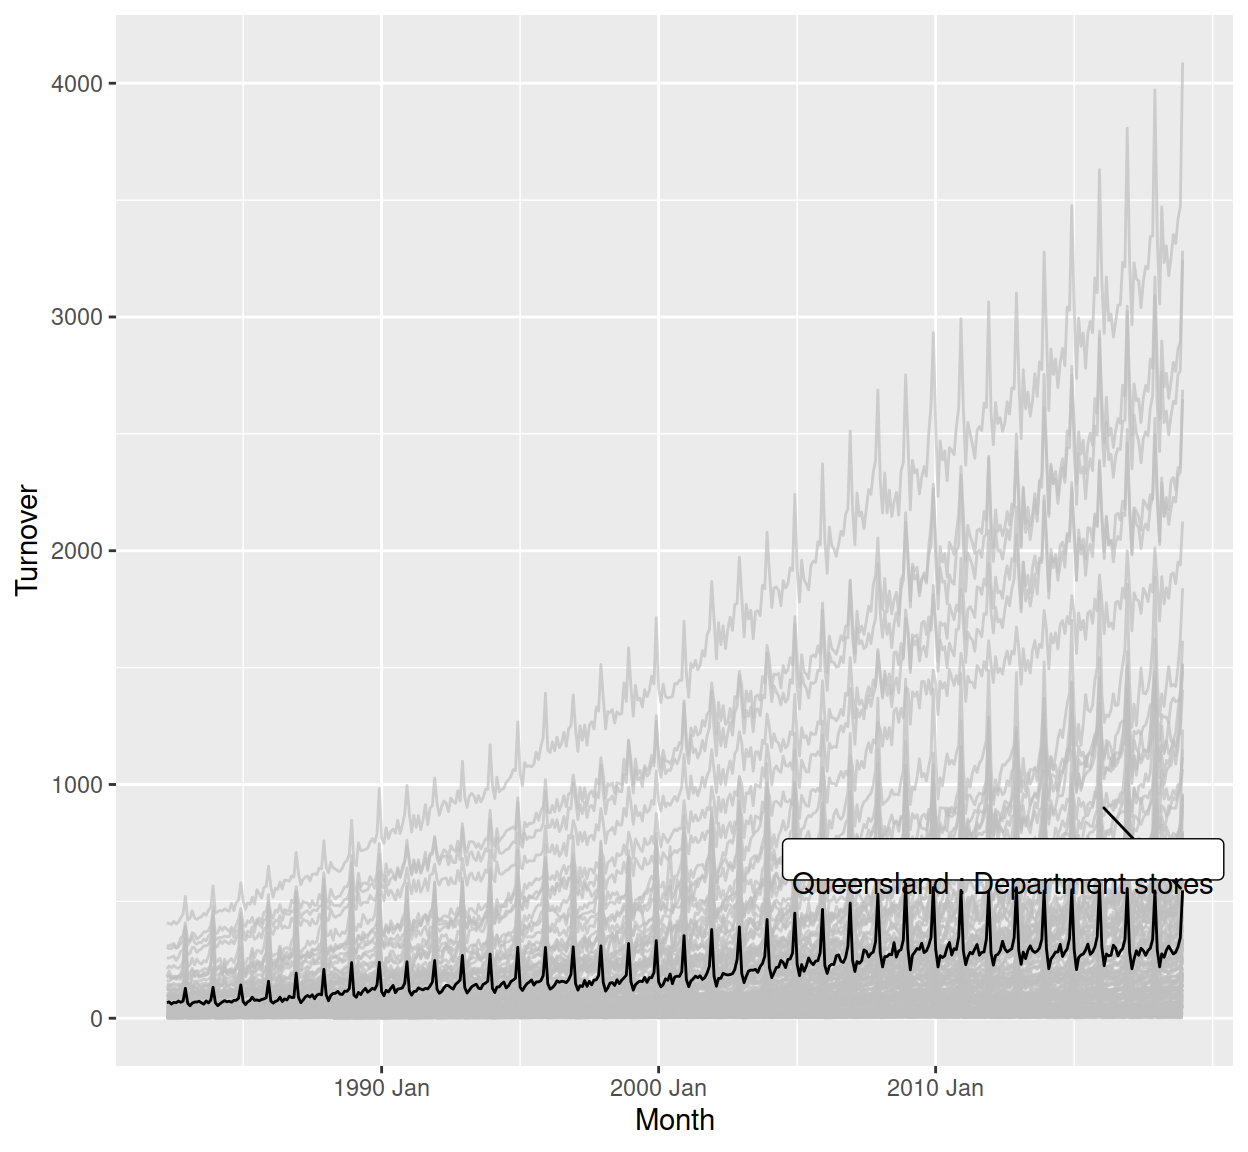
\includegraphics[width=.49\linewidth]{figure/highlight-retail-1} }\subfloat[\label{fig:highlight-retail-2}]{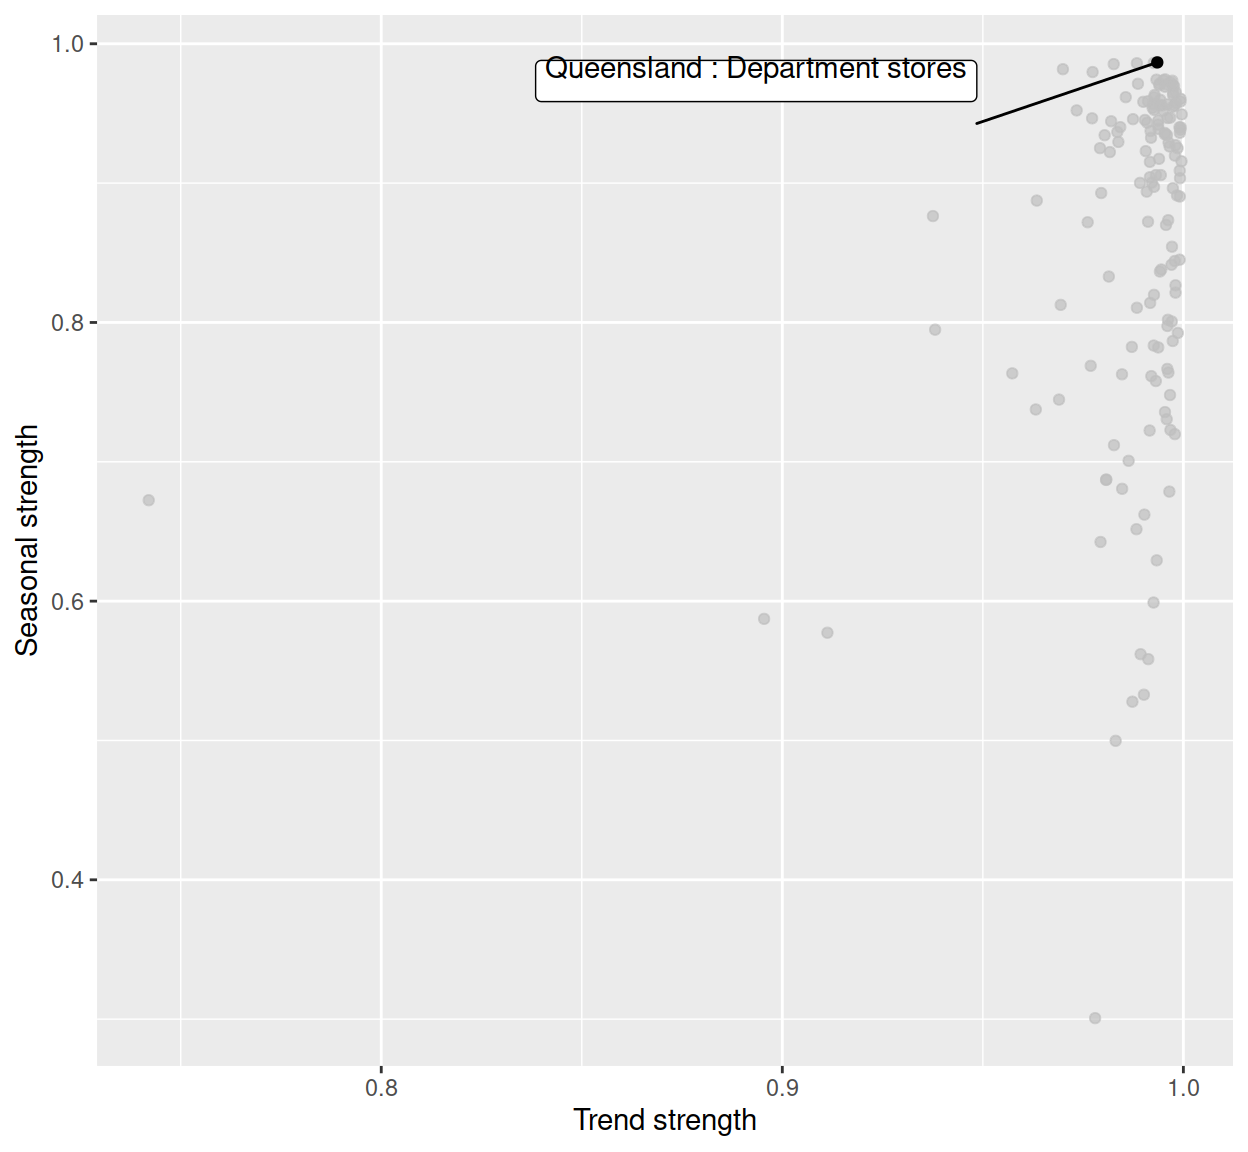
\includegraphics[width=.49\linewidth]{figure/highlight-retail-2} }

}

\caption{Plots for the \code{aus\_retail} data, with the series of strongest seasonal strength highlighted. (a) An overlaid time series plot. (b) A scatter plot drawn from their time series features, where each dot represents a time series from (a).}\label{fig:highlight-retail}
\end{figure}

Figure \ref{fig:highlight-retail} has also been highlighted to focus on the one series with the strongest seasonality. To create this highlighting, one needs to first filter the interesting series from the features table, and join back to the original \texttt{tsibble} in order to examine its trend in relation to others. This procedure can soon grow cumbersome if many series are to be explored. It illustrates a need to query interesting series on the fly. Although these two plots are static, we can consider them as linked views because the common \texttt{key} variables link between the two data tables producing the two plots. This motivates the work in this package, described in this paper, to enable interactivity of \texttt{tsibble} and \texttt{tsibble}-derived objects for rapid exploratory data analysis.

\hypertarget{overview-of-interactivity}{%
\section{Overview of interactivity}\label{overview-of-interactivity}}

There is a long history of interactive data visualization research and corresponding systems. Within R, the systems can be roughly divided into systems utilizing web technology and those that do not.

R \CRANpkg{shiny} (Chang et al. 2020) and \CRANpkg{htmlwidgets} (Vaidyanathan et al. 2019) provide infrastructure connecting R with HTML elements and JavaScript that support the interactivity. The \CRANpkg{htmlwidgets} package makes it possible to embed JavaScript libraries into R so that users are able to write only R code to generate web-based plots. Many JavaScript charting libraries have been ported to R as HTML widgets, including \CRANpkg{plotly} (Sievert 2020), \CRANpkg{rbokeh} (Hafen and Continuum Analytics, Inc. 2020), and \CRANpkg{leaflet} (J. Cheng, Karambelkar, and Xie 2019) for maps. Interactions between different widgets can be achieved with \CRANpkg{shiny} or \CRANpkg{crosstalk} (J. Cheng 2020). The \CRANpkg{crosstalk} extends \CRANpkg{htmlwidgets} with shared R6 instances to support linked brushing and filtering across widgets, without relying on \CRANpkg{shiny}.

Systems without the web technology include \CRANpkg{grDevices}, \CRANpkg{loon} (Waddell and Oldford 2020), based on Tcl/Tk, and \pkg{cranvas} (Xie, Hofmann, and Cheng 2014) based on Qt. They offer a wide array of pre-defined interactions, such as selecting and zooming, to manipulate plots via mouse action, keyboard strokes, and menus. The \pkg{cranvastime} package (X. Cheng, Cook, and Hofmann 2016) is an add-on to \pkg{cranvas}, which provides specialized interactions for temporal data, such as wrapping and mirroring.

The techniques implemented in the work described in this paper utilize web technology, including \CRANpkg{crosstalk}, \CRANpkg{plotly}, and R \CRANpkg{shiny}.

\hypertarget{using-a-shared-temporal-data-object-for-interactivity}{%
\section{Using a shared temporal data object for interactivity}\label{using-a-shared-temporal-data-object-for-interactivity}}

The \CRANpkg{tsibbletalk} package introduces a shared tsibble instance built on a \texttt{tsibble}. This allows for seamless communication between different plots of temporal data. The \texttt{as\_shared\_tsibble()} function turns a \texttt{tsibble} into a shared instance, \texttt{SharedTsibbleData}, which is a subclass of \texttt{SharedData} from \CRANpkg{crosstalk}. This is an R6 object driving data transmission across multiple views, due to its mutable and lightweight properties. The \CRANpkg{tsibbletalk} package aims to streamline interactive exploration of temporal data, with the focus of temporal elements and structured linking.

\hypertarget{linking-between-plots}{%
\subsection{Linking between plots}\label{linking-between-plots}}

As opposed to one-to-one linking, \CRANpkg{tsibbletalk} defaults to categorical variable linking, where selecting one or more observations in one category will broadcast to all other observations in this category. That is, linking is by key variables: within the time series plot, click on any data point, and the whole line will be highlighted in response. The \texttt{as\_shared\_tsibble()} uses \texttt{tsibble}'s \texttt{key} variables to achieve these types of linking.

The approach can also accommodate temporal data of nesting and crossing structures. These time series are referred to as hierarchical and grouped time series in the literature (Hyndman and Athanasopoulos 2017). The \texttt{aus\_retail} above is an example of grouped time series. Each series in the data corresponds to all possible combinations of the \texttt{State} and \texttt{Industry} variables, which means they are intrinsically crossed with each other. When one key variable is nested within another, such as regional areas within a state, this is considered to be a hierarchical structure.

The \texttt{spec} argument in \texttt{as\_shared\_tsibble()} provides a means to construct hybrid linking, that incorporates hierarchical and categorical linking. A symbolic formula can be passed to the \texttt{spec} argument, to define the crossing and/or nesting relationships among the key variables. Adopting Wilkinson and Rogers (1973)'s notation for factorial models, the \texttt{spec} follows the \texttt{/} and \texttt{*} operator conventions to declare nesting and crossing variables, respectively. The \texttt{spec} for the \texttt{aus\_retail} data is therefore specified as \texttt{State\ *\ Industry} or \texttt{Industry\ *\ State}, which is the default for the presence of multiple \texttt{key} variables. If there is a hierarchy in the data, using \texttt{/} is required to indicate the parent-child relation, for a strictly one directional \texttt{parent/child}.

To illustrate nesting and crossing we use the \texttt{tourism\_monthly} dataset (Tourism Research Australia 2020) packaged in \CRANpkg{tsibbletalk}. It contains monthly domestic overnight trips across Australia. The \texttt{key} is comprised of three identifying variables: \texttt{State}, \texttt{Region}, and \texttt{Purpose} (of the trip), in particular \texttt{State} nesting of \texttt{Region}, crossed together with \texttt{Purpose}. This specification can be translated as follows:

\begin{verbatim}
library(tsibble)
library(tsibbletalk)
tourism_shared <- tourism_monthly %>% 
  as_shared_tsibble(spec = (State / Region) * Purpose)
\end{verbatim}

\begin{figure}

{\centering 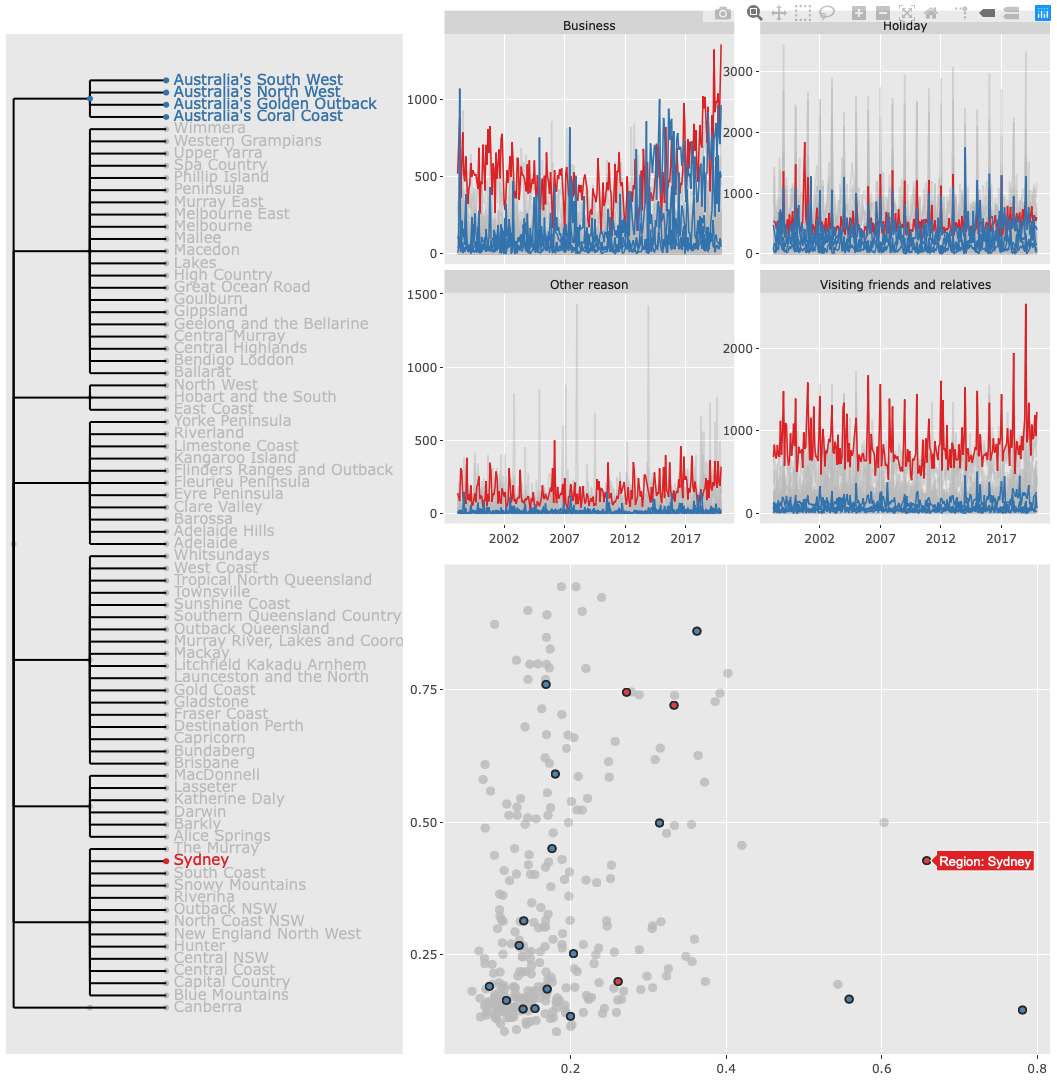
\includegraphics[width=\textwidth]{img/tourism-linking} 

}

\caption{Snapshot of exploring an ensemble of linked plots of the Australian tourism data, built on a \code{tourism\_shared} object. It also illustrates persistent linked brushing to compare two groups.}\label{fig:tourism-linking-fig}
\end{figure}

\noindent There is a three-level hierarchy: the root node is implicitly Australia, geographically disaggregated to states, and lower-level tourism regions. A new handy function \texttt{plotly\_key\_tree()} has been implemented to help explore the hierarchy. It interprets hierarchies in the shared tsibble's \texttt{spec} as a tree view, built with \CRANpkg{plotly}. The following code line produces the linked tree diagram (left panel of Figure \ref{fig:tourism-linking-fig}). The visual for the tree hierarchy detangles a group of related series and provides a bird's eye view of the data organization.

\begin{verbatim}
p_l <- plotly_key_tree(tourism_shared, height = 1100, width = 800)
\end{verbatim}

The tree plot provides the graphics skeleton, upon which the rest of the data plots can be attached. In this example, small multiples of line plots are placed at the top right of Figure \ref{fig:tourism-linking-fig} to explore the temporal trend across regions by the trip purpose. The shared tsibble data can be directly piped into \CRANpkg{ggplot2} code to create this.

\begin{verbatim}
library(ggplot2)
p_tr <- tourism_shared %>%
  ggplot(aes(x = Month, y = Trips)) +
  geom_line(aes(group = Region), alpha = .5, size = .4) +
  facet_wrap(~ Purpose, scales = "free_y") +
  scale_x_yearmonth(date_breaks = "5 years", date_labels = "%Y")
\end{verbatim}

These line plots are heavily overplotted. To tease apart structure in the multiple time series, the \texttt{features()} function computes interesting characteristics, including the measures of trend and seasonality. These are displayed in the scatterplot at the bottom right, where one dot represents one series.

\begin{verbatim}
library(feasts)
tourism_feat <- tourism_shared %>%
  features(Trips, feat_stl)
p_br <- tourism_feat %>%
  ggplot(aes(x = trend_strength, y = seasonal_strength_year)) +
  geom_point(aes(group = Region), alpha = .8, size = 2)
\end{verbatim}

There is one final step, to compose the three plots into an ensemble of coordinated views for exploration, shown in Figure \ref{fig:tourism-linking-fig}. (This is the interactive realization of Figure \ref{fig:highlight-retail}).

\begin{verbatim}
library(plotly)
subplot(p_l,
  subplot(
    ggplotly(p_tr, tooltip = "Region", width = 1100),
    ggplotly(p_br, tooltip = "Region", width = 1100),
    nrows = 2),
  widths = c(.4, .6)) %>%
  highlight(dynamic = TRUE)
\end{verbatim}

Since all plots are created from one shared tsibble data source, they are self-linking views. Nodes, lines, and points are hoverable and clickable. Given the \texttt{spec}, clicking either one element in any plot highlights all points that match the \texttt{Region} category, that is, categorical linking. Figure \ref{fig:tourism-linking-fig} is a static view of an interactive exploration. The steps in getting to this point were:

\begin{enumerate}
\def\labelenumi{\arabic{enumi}.}
\tightlist
\item
  A branch of the tree corresponding to Western Australia was first selected. (The names of the regions are a little odd, which is a quirk of the data set, but all four areas, Australia's South West, \ldots., correspond to tourist destinations in Western Australia. Hovering over the node on the branch brings up the state name.) This generated the response in the line plots and the scatterplot that colored corresponding time series and points as blue.
\item
  To enable persistent selection, in oder to compare regions or states, ``Shift'' and click on the tree was done, after switching the color to red. This generated the response that points and time series corresponding to Sydney were highlighted in red.
\item
  Hovering over the points brings up the label for Sydney.
\end{enumerate}

Domestic tourism sees Sydney as one of the most popular destinations in the realm of business and friends visiting over the years. Despite the relatively weaker performance in Western Australia, Australia's North West region sees a strongest upward trend in business, bypassing Sydney in some years.

In summary, shared tsibble data nicely bridges between the \CRANpkg{crosstalk} and \textbf{tidyverts} ecosystems for temporal data using the common ``key''. The \texttt{as\_shared\_tsibble()} provides a symbolic user interface for the effortless construction of a hybrid of hierarchical and categorical linking between plots. The \texttt{plotly\_key\_tree()} function, in turn, decodes the hierarchical specification to plot a tree for data overview and navigation, when accompanied by more detailed plots.

\hypertarget{slicing-and-dicing-time}{%
\subsection{Slicing and dicing time}\label{slicing-and-dicing-time}}

An important aspect of temporal data is the time context. Time has a cyclical structure, that may correspond to seasonal patterns to be discovered. The \texttt{index} component of the (shared) tsibble data forms the basis for exploring seasonality. To investigate for periodic or aperiodic patterns, series should be wrapped on themselves, where the index is broken into temporal components like quarter or day. We shall explore this with pedestrian traffic in Melbourne, Australia.

\begin{figure}

{\centering \subfloat[Initial overview state\label{fig:wrap-ped-1}]{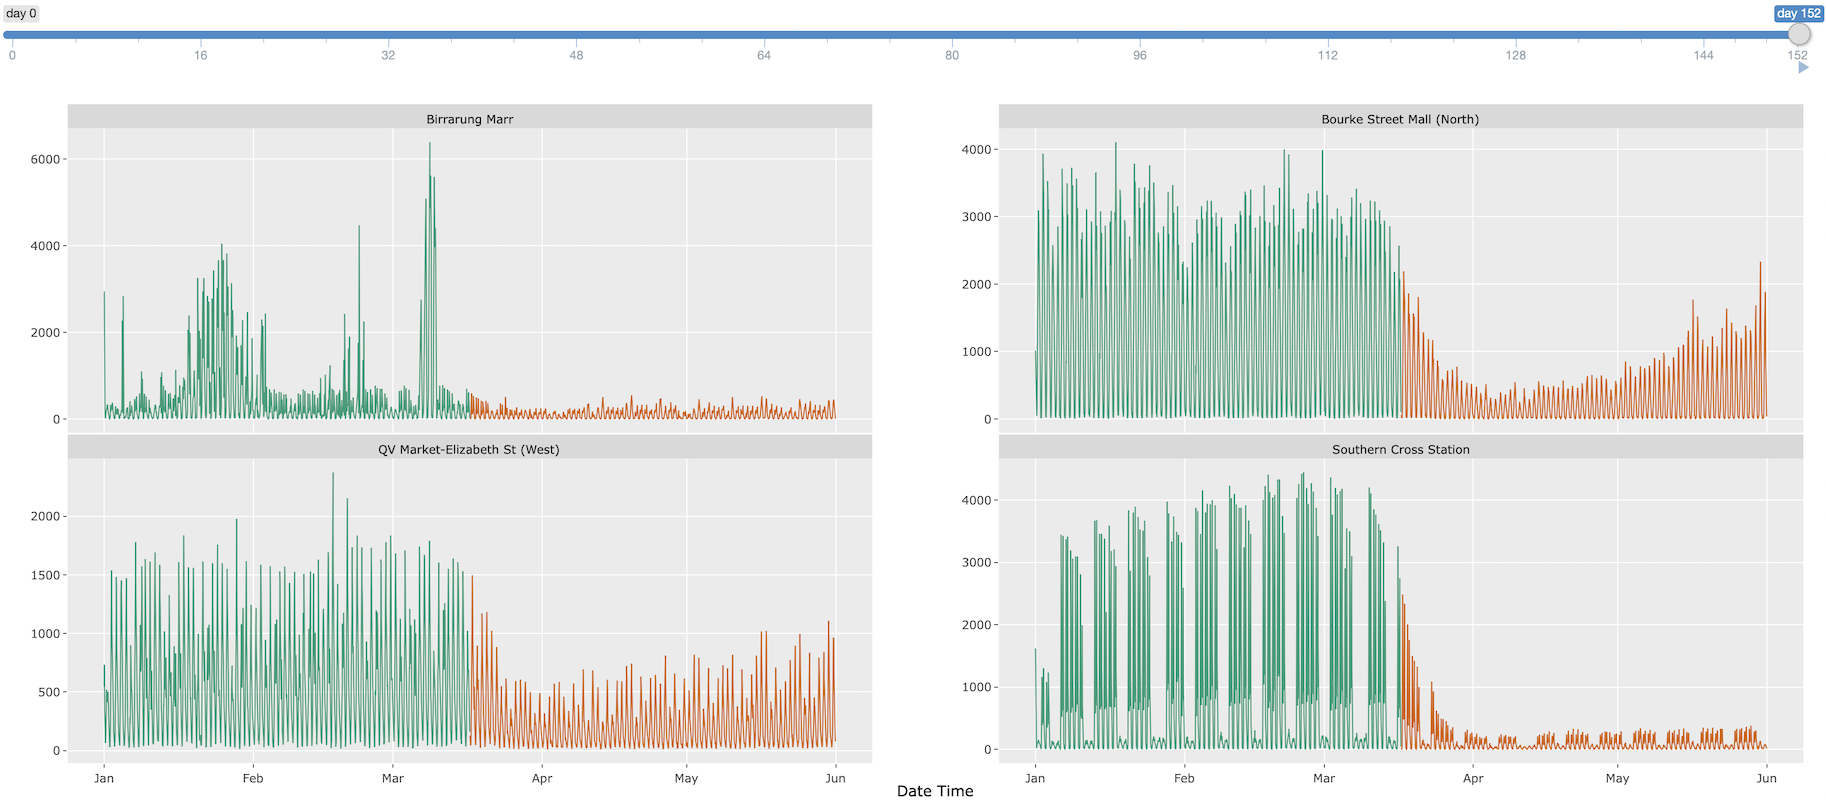
\includegraphics[width=\textwidth]{img/wrap-0} }\newline\subfloat[1-day state\label{fig:wrap-ped-2}]{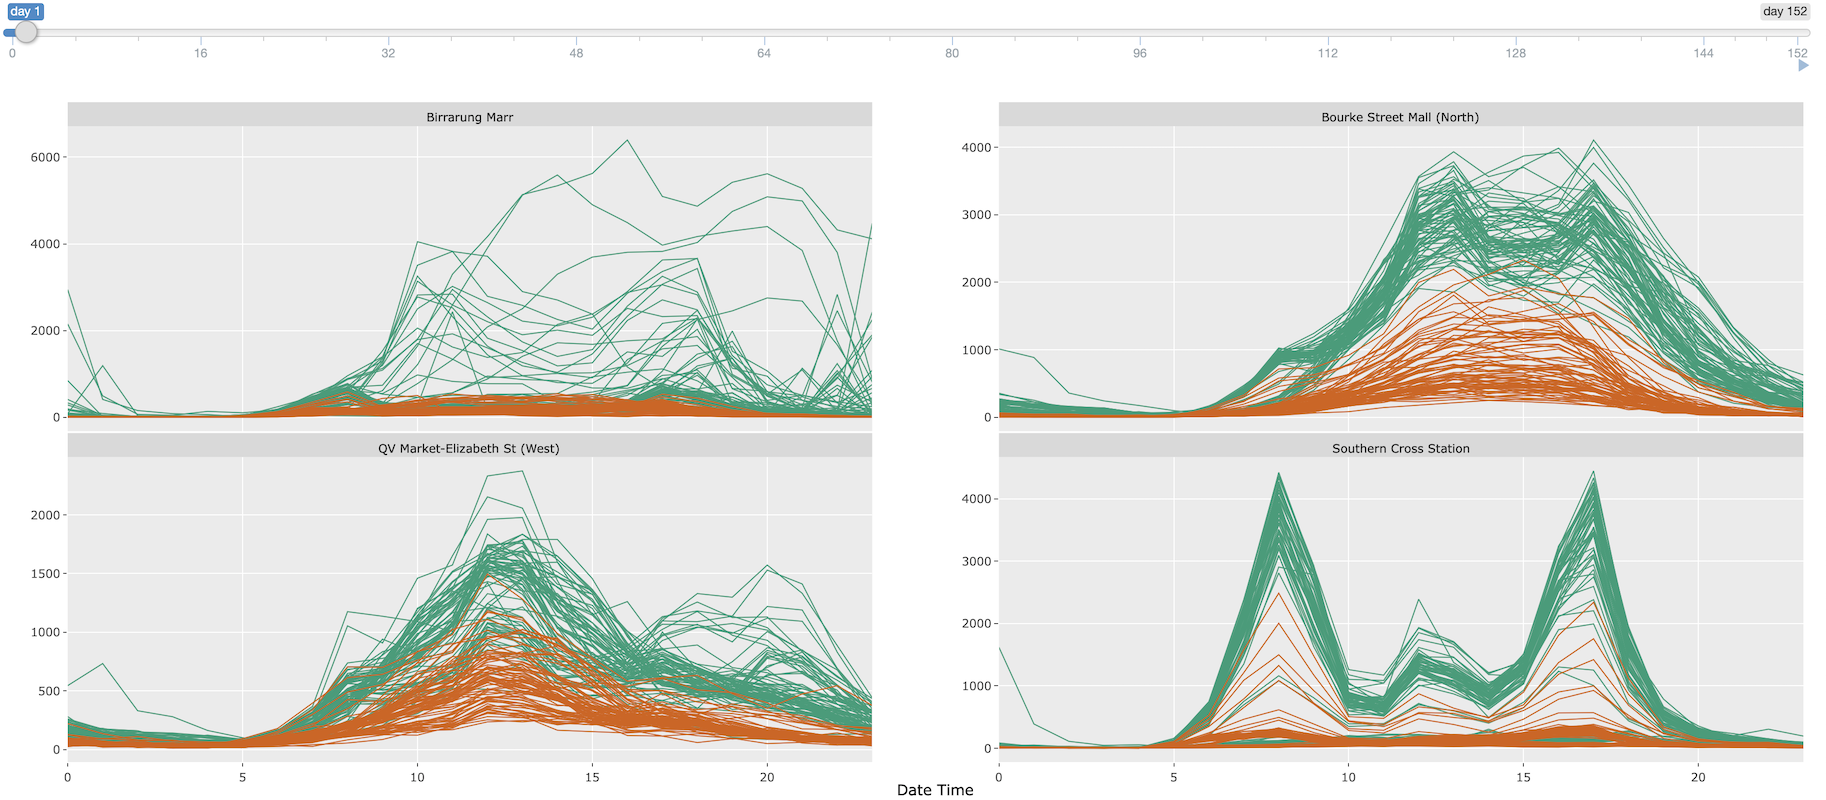
\includegraphics[width=\textwidth]{img/wrap-1} }\newline\subfloat[7-day state, anchoring to Monday\label{fig:wrap-ped-3}]{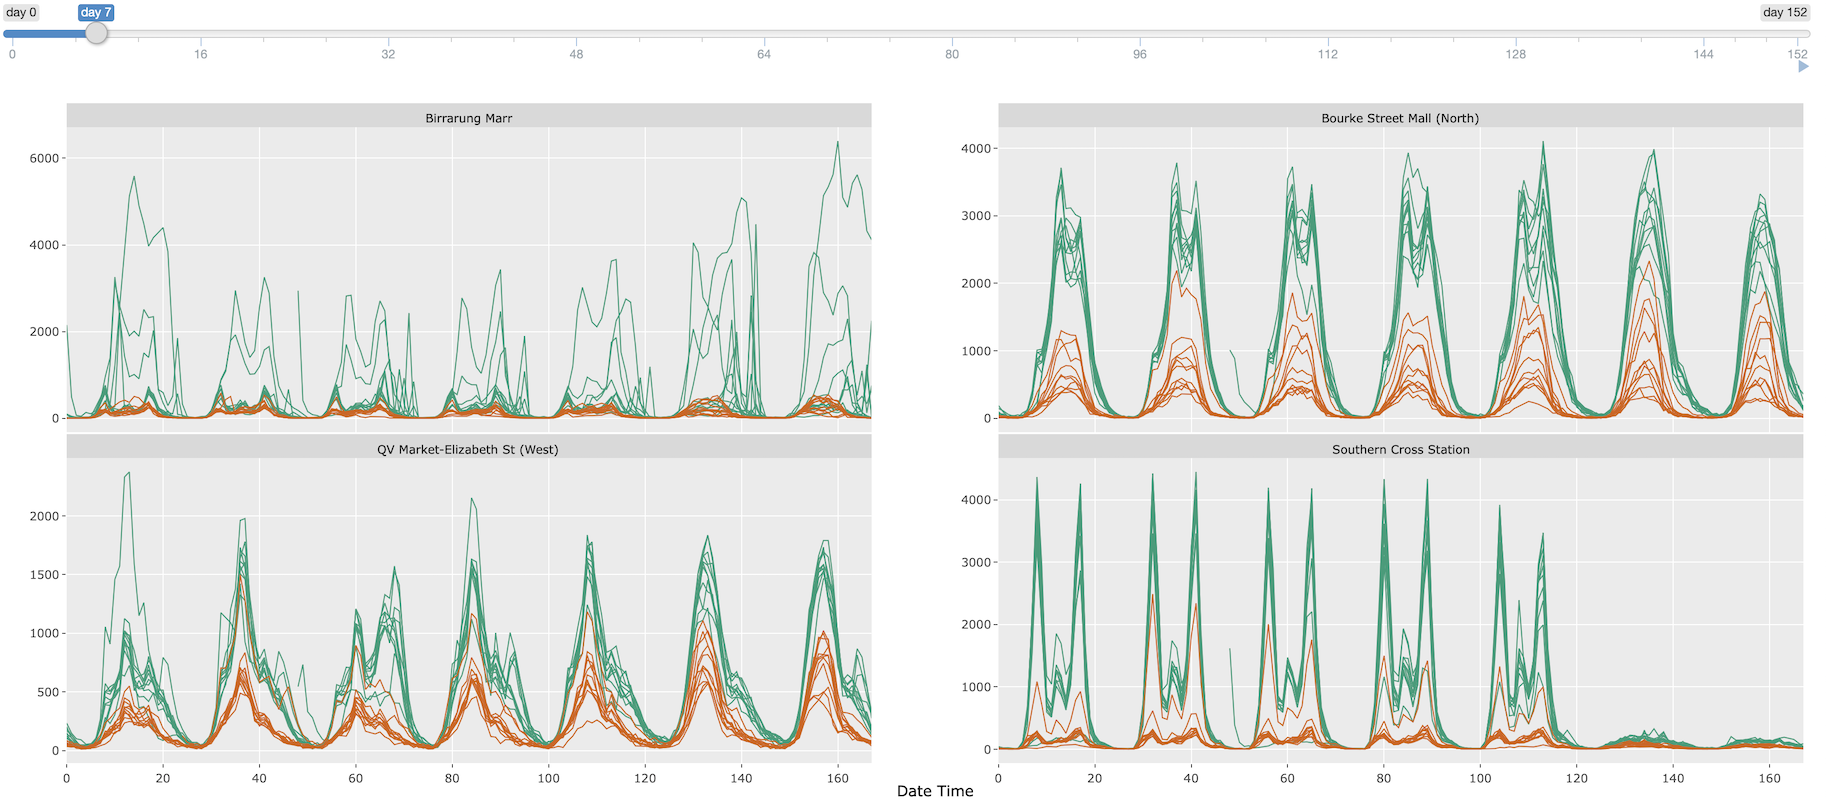
\includegraphics[width=\textwidth]{img/wrap-7} }

}

\caption{Snapshots wrapping after slicing the \code{pedestrian20} data at different intervals, (a) none, (b) daily and (c) weekly. This type of interaction is made possible with Shiny elements.}\label{fig:wrap-ped}
\end{figure}

The city of Melbourne has sensors installed at various locations, to record hourly counts of pedestrians, in order to capture the daily rhythms of the downtown (City of Melbourne 2020). Figure \ref{fig:wrap-ped} shows the first five months of 2020 foot traffic at four different locations, for three different time slices, daily, weekly and full five months. Plot \ref{fig:wrap-ped-1} shows hourly counts from January to May on an absolute timeline, facetted by locations. The stage 3 COVID-19 lockdown, on March 16, is marked by a change of color. (The pre-lockdown period is colored with dark green and lockdown with orange.) We can see a significant decline in foot traffic at all four locations. QV Market is less affected probably because this is a major produce market, an essential service that continued to operate. Bourke St, a major shopping center, sees a gradual uptick in the last weeks of the period indicating that people were getting back into the shops.

Figure \ref{fig:wrap-ped-2} and \ref{fig:wrap-ped-3} show the slicing and wrapping of the series into daily and weekly sections, respectively. Multiple seasonalities pop out. There tends to be a daily pattern, especially visible at the main train station, Southern Cross Station. There is also a weekday vs weekend pattern, also most visible at Southern Cross Station. These seasonal patterns are still present during the lockdown, but the magnitude is greatly reduced. Numbers are also down at the produce market and the shopping center. Birrarung Marr is the most affected. This is the location of special events, and it is clear that these have completely disappeared during the lockdown.

The wrapping procedure involves slicing the time index into seasonal periods of interest, and the result is diced time. For example, hourly pedestrian data can be decomposed into 24-hour blocks, which then overlays the counts for all respective days, as done in plot \ref{fig:wrap-ped-2}. For exploration, this slice position should be controlled interactively, so that many different slices can be examined rapidly. This can be achieved using shiny, with the functions provided in the \CRANpkg{tsibbletalk}.

This shiny module, decoupled to \texttt{tsibbleWrapUI()} and \texttt{tsibbleWrapServer()}, presents a clean interface and forms a reusable component that could be embedded in any shiny application. In general, a shiny module provides a vehicle for modularising shiny applications, relevant for both users and developers. As with all shiny modules, the first argument in both functions in \CRANpkg{tsibbletalk} requires a user-supplied id string that must be unique. The UI function \texttt{tsibbleWrapUI()} simply shows a slider that animates or controls the number of periods to be diced. The workhorse is the server function \texttt{tsibbleWrapServer()}, encapsulating the algorithm that transforms data and sends messages to update the plot accordingly. The \texttt{plot} argument expects a \texttt{ggplot} or \texttt{plotly} object, where one can plot data using either lines or other graphical elements (such as boxplots). As the function name suggests, a (shared) tsibble is needed to start the engine, so that the time \texttt{index} can be retrieved for dissection. The \texttt{period} option semantically takes a desired number of seasonal periods to be shifted, for example data shifted by ``1 day'', ``2 days'', or ``1 week'', etc. In other words, the \texttt{period} defines the grind level. For date-times (represented by \texttt{POSIXt}), the granularity ranges from fine ``day'' to a much coarser ``year''. The following code snippet generates Figure \ref{fig:wrap-ped}. The creation of the \texttt{pedestrian20} data is available in supplementary R files.

\begin{verbatim}
library(shiny)
p_line <- pedestrian20 %>%
  ggplot(aes(x = Date_Time, y = Count, colour = Lockdown)) +
  geom_line(size = .3) +
  facet_wrap(~ Sensor, scales = "free_y") +
  labs(x = "Date Time") +
  scale_colour_brewer(palette = "Dark2") +
  theme(legend.position = "none")

ui <- fluidPage(
  tsibbleWrapUI("dice")
)
server <- function(input, output, session) {
  tsibbleWrapServer("dice", ggplotly(p_line, height = 700), period = "1 day")
}
shinyApp(ui, server)
\end{verbatim}

Figure \ref{fig:wrap-ped-1} corresponds to the initial state, with the slider incremented by 1-day units. The ``play'' button near the end of the slider can automatically animate the slicing and dicing process, walking the viewer through all 24 hours of the 152 days. Alternatively, users can drag the slider to examine selected slices.

In response to the slider input, the plot will be updated and loaded with newly transformed data. At its core, keeping the application as performant as possible is the top priority. Without completely redrawing the plot, the \texttt{plotlyProxy()} react method is invoked internally for talking to shiny. The underlying tsibble data is being called back and processed in R. Only transformed data gets fed back to the shiny server, for updating with resetting the x-axis ranges and breaks. The other plot configurations, such as marks, y-axes, and layouts, are cached and used as is.

The new shiny module exploits the temporal aspect for a tsibble object, available through the \texttt{index} attribute. It allows users to slide through relative periods to digest seasonal behaviors, with a nimble user experience.

\hypertarget{summary}{%
\section{Summary}\label{summary}}

At the heart of the \CRANpkg{tsibbletalk} package is a blending of the best bits from \CRANpkg{tsibble}, \CRANpkg{crosstalk}, \CRANpkg{plotly}, and \CRANpkg{shiny}.

The \texttt{as\_shared\_tsibble()} turns a \texttt{tsibble} object to a shared data class, with an option to express any nesting and crossing structures from the \texttt{key} attribute. If nesting is found in the data, the \texttt{plotly\_key\_tree()} creates an interactive hierarchical tree to help with the data overview. This sets the stage for hierarchical and categorical linking between multiple views from one shared tsibble.

A new shiny module, \texttt{tsibbleWrapUI()} and \texttt{tsibbleWrapServer()}, provides a lens for looking at temporal aspects of a \texttt{tsibble}, in particular seasonal or cyclical variations. The slicing and dicing technique efficiently wrap time lines for user-defined plots. The \texttt{plotlyProxy()} react method makes it possible to send wrapped data to the server and amend the plot straight way.

\hypertarget{references}{%
\section*{References}\label{references}}
\addcontentsline{toc}{section}{References}

\hypertarget{refs}{}
\begin{CSLReferences}{1}{0}
\leavevmode\vadjust pre{\hypertarget{ref-R-shiny}{}}%
Chang, Winston, Joe Cheng, JJ Allaire, Yihui Xie, and Jonathan McPherson. 2020. \emph{Shiny: Web Application Framework for r}. \url{https://CRAN.R-project.org/package=shiny}.

\leavevmode\vadjust pre{\hypertarget{ref-R-crosstalk}{}}%
Cheng, Joe. 2020. \emph{Crosstalk: Inter-Widget Interactivity for HTML Widgets}. \url{https://CRAN.R-project.org/package=crosstalk}.

\leavevmode\vadjust pre{\hypertarget{ref-R-leaflet}{}}%
Cheng, Joe, Bhaskar Karambelkar, and Yihui Xie. 2019. \emph{Leaflet: Create Interactive Web Maps with the JavaScript 'Leaflet' Library}. \url{https://CRAN.R-project.org/package=leaflet}.

\leavevmode\vadjust pre{\hypertarget{ref-cheng_enabling_2016}{}}%
Cheng, Xiaoyue, Dianne Cook, and Heike Hofmann. 2016. {``Enabling Interactivity on Displays of Multivariate Time Series and Longitudinal Data.''} \emph{Journal of Computational and Graphical Statistics} 25 (4): 1057--76. \url{https://www.tandfonline.com/doi/full/10.1080/10618600.2015.1105749}.

\leavevmode\vadjust pre{\hypertarget{ref-ped}{}}%
City of Melbourne. 2020. \emph{Pedestrian Volume in Melbourne}. City of Melbourne, Australia. \url{http://www.pedestrian.melbourne.vic.gov.au}.

\leavevmode\vadjust pre{\hypertarget{ref-R-rbokeh}{}}%
Hafen, Ryan, and Continuum Analytics, Inc. 2020. \emph{Rbokeh: R Interface for Bokeh}. \url{https://CRAN.R-project.org/package=rbokeh}.

\leavevmode\vadjust pre{\hypertarget{ref-fpp}{}}%
Hyndman, Rob J, and George Athanasopoulos. 2017. \emph{Forecasting: Principles and Practice}. Melbourne, Australia: OTexts. \href{https://OTexts.org/fpp2}{OTexts.org/fpp2}.

\leavevmode\vadjust pre{\hypertarget{ref-R-fable}{}}%
O'Hara-Wild, Mitchell, Rob Hyndman, and Earo Wang. 2020a. \emph{Fable: Forecasting Models for Tidy Time Series}. \url{https://CRAN.R-project.org/package=fable}.

\leavevmode\vadjust pre{\hypertarget{ref-R-feasts}{}}%
---------. 2020b. \emph{Feasts: Feature Extraction and Statistics for Time Series}. \url{https://CRAN.R-project.org/package=feasts}.

\leavevmode\vadjust pre{\hypertarget{ref-R-tsibbledata}{}}%
---------. 2020c. \emph{Tsibbledata: Diverse Datasets for 'Tsibble'}. \url{https://CRAN.R-project.org/package=tsibbledata}.

\leavevmode\vadjust pre{\hypertarget{ref-plotly2020}{}}%
Sievert, Carson. 2020. \emph{Interactive Web-Based Data Visualization with r, Plotly, and Shiny}. Chapman; Hall/CRC. \url{https://plotly-r.com}.

\leavevmode\vadjust pre{\hypertarget{ref-tourism}{}}%
Tourism Research Australia. 2020. \emph{Australian Domestic Overnight Trips}. Tourism Research Australia, Australia. \url{https://www.tra.gov.au}.

\leavevmode\vadjust pre{\hypertarget{ref-unwin_ensemble_2018}{}}%
Unwin, Antony, and Pedro Valero-Mora. 2018. {``Ensemble {Graphics}.''} \emph{Journal of Computational and Graphical Statistics} 27 (1): 157--65. \url{https://www.tandfonline.com/doi/full/10.1080/10618600.2017.1383264}.

\leavevmode\vadjust pre{\hypertarget{ref-R-htmlwidgets}{}}%
Vaidyanathan, Ramnath, Yihui Xie, JJ Allaire, Joe Cheng, and Kenton Russell. 2019. \emph{Htmlwidgets: HTML Widgets for r}. \url{https://CRAN.R-project.org/package=htmlwidgets}.

\leavevmode\vadjust pre{\hypertarget{ref-R-loon}{}}%
Waddell, Adrian, and R. Wayne Oldford. 2020. \emph{Loon: Interactive Statistical Data Visualization}. \url{https://CRAN.R-project.org/package=loon}.

\leavevmode\vadjust pre{\hypertarget{ref-wang2020tsibble}{}}%
Wang, Earo, Dianne Cook, and Rob J Hyndman. 2020. {``A New Tidy Data Structure to Support Exploration and Modeling of Temporal Data.''} \emph{Journal of Computational and Graphical Statistics} 29 (3): 466--78. \url{https://doi.org/10.1080/10618600.2019.1695624}.

\leavevmode\vadjust pre{\hypertarget{ref-wickham2014tidy}{}}%
Wickham, Hadley. 2014. {``Tidy Data.''} \emph{Journal of Statistical Software} 59 (10): 1--23.

\leavevmode\vadjust pre{\hypertarget{ref-Wickham2019}{}}%
Wickham, Hadley, Mara Averick, Jennifer Bryan, Winston Chang, Lucy D'Agostino McGowan, Romain François, Garrett Grolemund, et al. 2019. {``Welcome to the Tidyverse.''} \emph{Journal of Open Source Software} 4 (43): 1686. \url{https://doi.org/10.21105/joss.01686}.

\leavevmode\vadjust pre{\hypertarget{ref-Wilkinson1973}{}}%
Wilkinson, G. N., and C. E. Rogers. 1973. {``Symbolic Description of Factorial Models for Analysis of Variance.''} \emph{Journal of the Royal Statistical Society. Series C (Applied Statistics)} 22 (3): 392--99. \url{http://www.jstor.org/stable/2346786}.

\leavevmode\vadjust pre{\hypertarget{ref-xie_reactive_2014}{}}%
Xie, Yihui, Heike Hofmann, and Xiaoyue Cheng. 2014. {``Reactive Programming for Interactive Graphics.''} \emph{Statistical Science} 29 (2): 201--13. \url{http://projecteuclid.org/euclid.ss/1408368571}.

\end{CSLReferences}

\bibliography{tsibbletalk.bib}

\address{%
Earo Wang\\
The University of Auckland\\%
Department of Statistics\\
%
%
%
\href{mailto:earo.wang@auckland.ac.nz}{\nolinkurl{earo.wang@auckland.ac.nz}}%
}

\address{%
Dianne Cook\\
Monash University\\%
Department of Econometrics and Business Statistics\\
%
%
%
\href{mailto:dicook@monash.edu}{\nolinkurl{dicook@monash.edu}}%
}
